\documentclass[a4paper, 12 pt, conference]{ieeeconf}  % 
\IEEEoverridecommandlockouts                              % This command is only
% needed if you want to
% use the \thanks command

\overrideIEEEmargins
% See the \addtolength command later in the file to balance the column lengths
% on the last page of the document

% Pacote de acentuação
\usepackage[brazil]{babel}
\usepackage[utf8]{inputenc}

% The following packages can be found on http:\\www.ctan.org
\usepackage{graphics} % for pdf, bitmapped graphics files
\usepackage{epsfig} % for postscript graphics files
%\usepackage{mathptmx} % assumes new font selection scheme installed
%\usepackage{mathptmx} % assumes new font selection scheme installed
\usepackage{amsmath} % assumes amsmath package installed
\usepackage{amssymb}  % assumes amsmath package installed

\usepackage[]{todonotes} % adicionar parâmetro [disable] para ocultar os comentários
\usepackage{xspace} % usado nos comentários
\usepackage[normalem]{ulem}
\usepackage{hyperref}
\hypersetup{
	colorlinks=true,
	linkcolor=blue,
	filecolor=magenta,      
	urlcolor=cyan,
}

\newcounter{todocounter}
\setlength{\marginparwidth}{2cm}
\reversemarginpar
\newcommand{\nota}[1]{\xspace\stepcounter{todocounter}\todo[fancyline]{\thetodocounter: #1}}
\newcommand{\notain}[2]{\stepcounter{todocounter}\todo[inline]{\thetodocounter: (#1) #2}}

\title{\LARGE \bf
Classificação de emoções por meio de expressões faciais em sala de aula
}

\author{Marcus V. S. Maziero$^{1}$e Paulo R. K. Nakaima$^{2}$
\thanks{$^{1}$Marcus V. S. Maziero e $^{2}$Paulo R. K. Nakaima estão vinculados à Universidade Tecnológica Federal do Paraná, Av. Alberto Carazzai, 1640, Cornélio Procópio, Brasil. 
        {\tt\small marcus.maziero$@$outlook.com, nakaima$@$alunos.utfpr.edu.br}}%
}


\begin{document}


\maketitle
\thispagestyle{empty}
\pagestyle{empty}


%%%%%%%%%%%%%%%%%%%%%%%%%%%%%%%%%%%%%%%%%%%%%%%%%%%%%%%%%%%%%%%%%%%%%%%%%%%%%%%%
\begin{abstract}
Procura-se neste trabalho realizar breve revisão bibliográfica sobre problema de reconhecimento de expressões faciais em sala de aula para melhorar a qualidade de ensino. Na sequência será realizado um laboratório para demonstrar a aplicação de técnicas de aprendizado de máquina para a solução do problema. Busca-se abordar de forma introdutória e simplificada o tema para fundamentar trabalhos futuros.
\end{abstract}

\begin{keywords}
Inteligencia Artificial, Emoções, Imagens, Machine Learning.
\end{keywords}


%%%%%%%%%%%%%%%%%%%%%%%%%%%%%%%%%%%%%%%%%%%%%%%%%%%%%%%%%%%%%%%%%%%%%%%%%%%%%%%%
\section{INTRODUÇÃO}
O reconhecimento de expressões faciais são um campo especifico e instigante da área de Inteligencia Artificial (IA), conforme descreve \cite{murtaza:2019}, pois possibilita encontrar e rastrear movimentos incomuns na face das pessoas.

Com o rastreamento desses dados é possível por intermédio classificar as mesmas e compreender como as emoções afetam as tomadas de decisões, conforme \cite{hieida:2018} é um ponto instigante a ser aprofundado.
Em uma perspectiva de utilizar e melhorar o desempenho das aplicações que reconhecem e classificam expressões faciais é utilizado já por algumas empresas o Machine Learning (ML) termo em inglês que remete ao aprendizado de maquina, conforme apresenta \cite{ray:2019}, a utilização do ML já uma prática familiar em algumas empresas.

Sendo assim a presente pesquisa foi desenvolvida com o intuito de auxiliar os campos pesquisados e apresentar resultados de práticas e técnicas de reconhecimento facial.

\section{CONTEXTO}
A classificação de emoções por reconhecimento facial é algo que pode ser utilizado para favorecer a área escolar, conforme \cite{sahla:2016}, as emoções podem descrever a maturidade de aprendizado do discente e como o mesmo está diante dos ensinos propostos. Com isso essa classificação auxilia o docente para aumentar o desempenho da sua turma de alunos, melhorando assim o ensino.

Esse tipo de classificação também pode ser usado para fins sociais e comerciais para aumentar desempenhos de vendas e melhorar a abordagem das empresas relacionadas as frentes descritas como apresenta \cite{ozcan:2019} em sua pesquisa. Dessa forma é possível dizer que a classificações de expressões faciais podem auxiliar diversas áreas e que com o avanço desta resulta em diversas melhorias para a educação, comércio, medicina e atividades sociais.

\section{OBJETIVOS}
Classificar expressões faciais a partir de imagens utilizando técnicas de processamento de imagens.
Apresentar protótipo de classificador de expressões facias visando desenvolver aplicação para professores avaliarem o engajamento dos alunos durante a aula.

\section{TRABALHOS RELACIONADOS}
Em \cite{piotto:2016} é apresentada uma abordagem para extração de características de imagens visando o melhoramento da acurácia para o reconhecimento facial. Esta abordagem é baseada na teoria de redes complexas a qual fornece as medidas para remoção de conexões menos significativas para o processo de aprendizado de máquina. Com esse procedimento foi possível obter acurácia de 95\% e 96.3\% nas bases \textit{Caltech Face Dataset} (CFD)  e \textit{Head Pose Image base} (HPI).

Em \cite{sahla:2016} criam um sistema para analizar emoções em sala de aula. Aplicam redes neurais convolucionais (\textit{Convolutional Neural Network} - CNN) para classificar as expressões faciais dos alunos e professor. A aula é gravada em vídeo, na sequência esse é convertido em \textit{frames}; utilizam o algoritmo \textit{Viola-Jones} para detecção facial, ao resultado é aplicado o descritor de texturas \textit{Local Binary Pattern} (LBP), por fim, é utilizado CNN para classificação das emoções. O sistema foi testado com 105 imagens retiradas das bases CK, JAFFE e \textit{google images} as quais incluem fotos de pessoas sozinhas ou em grupos. As expressões foram classificadas como raiva, nojo, felicidade, neutralidade, supresa, medo e tristeza. Obteve, respectivamente percentual de acerto de: 33.3\%, 46,6\%, 60\%, 46,6\%, 0\%, 33,3\%, 53,3\%. No teste com a gravação em vídeo o sistema acertou 80,9\% em média e erro de 19,1\%. 

Em \cite{cruz:2019} apresenta uma pesquisa de reconhecimento de emoções humanas por imagens faciais, com a abordagem \textit{Single Shot Facial Expression Recognition} (SSFER), demonstra que o método MMOD-CNN foi o que apresentou melhor acurácia 91.89\%, para comprovar é apresentado o resultado de experimentos combinando CNN e classificador, com cinco CNN e quatro classificadores, são eles VGGNet, InceptionResNetV2, InceptionV3, MobileNetV2, ResidualNet, Softmax, SVM, Random Forest e KNN respectivamente, a pesquisa também demonstra um experimento real com vinte e sete estudantes do ensino médio utilizando do MMOD-CNN para reconhecer as emoções dos alunos.


\section{METODOLOGIA}
\subsection{Ambiente de Software}
Para realizar o laboratório foi utilizado de algumas tecnologias e ferramentas são elas: 
\begin{itemize}
	\item \textit{Scikit}: é uma ferramenta de código aberto, simples e eficaz na análise de dados, acessivel e reutilizavel por vários contextos \cite{scikit-learn}. O projeto foi iniciado em 2007 com por intermédio de um projeto da Google Summer of Code, atualmente é mantido pela comunidade
	\item \textit{Python}: é uma linguagem de programação em script´s, interpretada, de código aberto e rápida, mantido pela comunidade e administrada pela Python Software Foundation. Diversas empresas já utilizam dela, como Google, YouTube e EVE Online.
\end{itemize}

\subsection{Base de dados}
Foi selecionada a base de imagens CKPLUS48. A qual pode ser encontrada em: https://www.kaggle.com/shawon10/ckplus. Contém 750 imagens de rostos em escalas de cinza com as expressões de raiva, nojo, desprezo, medo, felicidade, tristeza e surpresa. Para este laboratório foram selecionadas apenas as expressões raiva, medo, felicidade, tristeza e surpresa.

\subsection{Extração de características}

Para extração de características foi utilizado os descritores Local Binary Patterns (LBP) e o Gabor.

Sendo que o primeiro extrai 256 características de textura é não paramétrico, possui baixo custo de processamento \cite{rajan:19}. Seu funcionamento consiste em dividir a imagem em sub-blocos sendo que para cada sub-bloco é calculado o histograma, o vetor de características é formado com a concatenação desses histogramas \cite{rajan:19}.
Sendo que o segundo gera filtros com ondas senoidal, com os eixos desta onda busca encontrar a Gaussiana e assim manter uma proporção constante na imagem, para no final do processo gerar contornos e texturas para obter dados\cite{lima:2016}.Neste laboratório o Gabor extrai 60 características de textura como linhas e contornos nas imagens.
 
 Os arquivos finais podem ser encontrados em: \url{encurtador.com.br/gnDOZ}.

\subsection{Seleção dos classificadores e técnica de amostragem}
Os classificadores foram selecionados com base no trabalho de \cite{rajan:19}, o qual indica quais foram os mais utilizados em problemas de reconhecimento de expressões faciais (Facial Expression Recognition - FER), sendo eles:
\begin{itemize}
	\item \textit{Regressão Logística (Logistic Regression - LR)}: produz a partir de um conjunto de dados, modelos que permitem a predição por variaveis categóricas
	\item \textit{ K-Nearest Neighbors - (KNN)}: procura o vizinho K mais próximo de um dado ponto no espaço do conjunto de dados.
	\item \textit{Máquina de Vetores Suporte (Support Vectors Machine - SVM)}: é uma maquina de entrada e saida onde os dados que são enviados como entrada são mapeadas em um espaço multidimensional e encontra um hiperplano que separa os dados de entrada.
	\item \textit{Rede Perceptron Multicamadas (Multi-Layer Perceptron - MLP)}: é uma rede neural com camadas onde os números de neurônios são indeterminados, sendo assim não é possível prever a saída intermediaria entre as camadas.
	
\end{itemize}

 Para os experimentos executados nas seções seguintes o conjunto de dados foram divididos em 80\% para treino e 20\% para teste. A seleção desses subconjuntos foram feitos de modo aleatório com o número gerador  (\textit{seed}) 327 para possível reprodução dos experimentos.

\subsection{Seleção da técnica de normalização}

A partir dos arquivos gerados com os descritores foram alternadas as técnicas de normalização para verificar qual delas atinge melhor resultado para acurácia, métrica que calcula a razão entre quantidade de predições corretas e a quantidade de predições realizadas. 

As técnicas de normalização testadas foram:
\begin{itemize}
	\item \textit{Min-Max}: consiste em transformar cada característica com valor mínimo em 0 e os valores máximos em 1, sendo que o restante é transformado em um valor decimal entre 0 e 1.
	\item \textit{Standard}: são calculados a média e o desvio padrão da conjunto de amostras, em seguida é subtraída de cada amostra a média, o resultado então é divido pelo desvio padrão.
	\item \textit{Max Absolute}:é uma técnica parecida com o Min-Max porém, somente os valores absolutos e positivos são mapeados entre 0 e 1.
	\item \textit{Robust}: as estatísticas de mapeamento ocorrem pela escala de percentil, sendo assim aumenta a margem de onde estão os valores dos dados podendo ser até negativo, exemplo: -3 a 2.
\end{itemize}

\subsubsection{Descritor LBP}
A base CKPLUS com o descritor LBP apresentou pequena variação nos resultados como podem ser vistas na Figura~\ref{fig:bar_norm_all}.

\begin{figure}[!htbp]
	\centering
	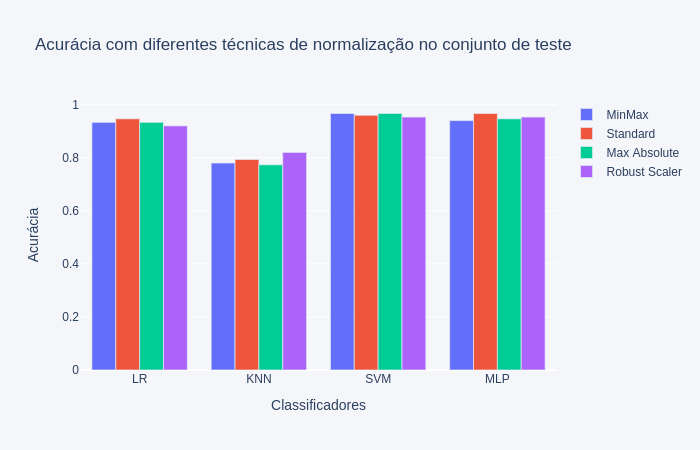
\includegraphics[width=1.0\linewidth,clip=true,trim=0cm 0cm 0cm 0cm, keepaspectratio=true]{bar_norm_all.png}
	\caption{Comparação de técnicas de normalização com descritor LBP.}
	\label{fig:bar_norm_all}
\end{figure}

Os classificadores MLP, SVM obtiveram os melhores resultados, 97\% de acurácia. Os piores resultados foram obtidos pelo classificador KNN, 77\%.

\subsubsection{Descritor Gabor}
Foram mantidos os classificadores e métrica utilizados no último experimento. Nenhum dos classificadores obtiveram 50\% de acurácia. Os resultados podem ser vistos na Figura~\ref{fig:bar_norm_all_gabor}.

\begin{figure}[!htbp]
	\centering
	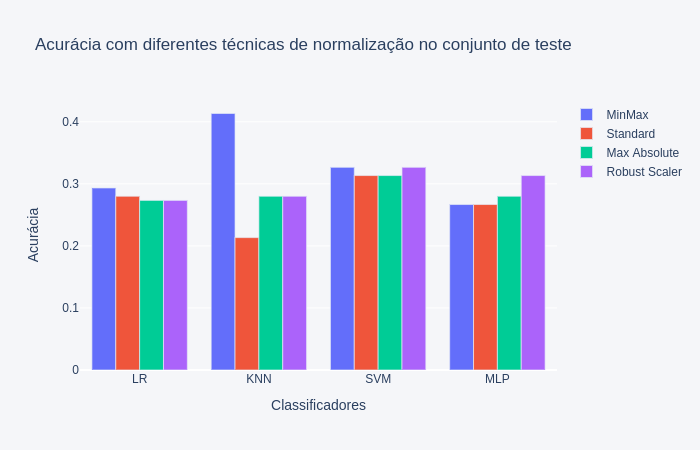
\includegraphics[width=1.0\linewidth,clip=true,trim=0cm 0cm 0cm 0cm, keepaspectratio=true]{bar_norm_all_gabor.png}
	\caption{Comparação de técnicas de normalização com descritor Gabor.}
	\label{fig:bar_norm_all_gabor}
\end{figure}

Pode-se observar que a técnica de normalização Min-Max, atrelado ao classificador KNN obteve o melhor resultado deste experimento, 41\%. Observa-se também que ocorre uma alta discrepância sobre os resultado obtidos entre os descritores LBP e Gabor.

\subsection{Redução de dimensionalidade}
\subsubsection{Descritor LBP}
Em seguida buscou-se reduzir a dimensão do conjunto de dados de modo a reter 90\% de variância. Primeiramente os dados foram normalizados utilizando a técnica \textit{Standard}, pois obteve resultado levemente superior no experimento anterior.

Com a técnica PCA para redução de dimensionalidade foi selecionado o menor número de componentes que retinha 90\% de variância. Foi possível reduzir de 256 para 133 característica. Ver Figura~\ref{fig:points_pca_lbp}. 

\begin{figure}[!htbp]
	\centering
	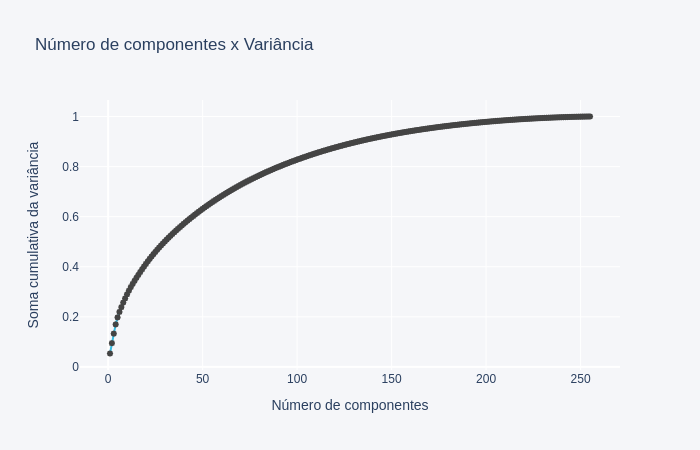
\includegraphics[width=1.0\linewidth,clip=true,trim=0cm 0cm 0cm 0cm, keepaspectratio=true]{points_pca_lbp.png}
	\caption{Selecionar o menor número de componentes retendo 90\% de variância.}
	\label{fig:points_pca_lbp}
\end{figure}

\subsubsection{Descritor Gabor}
Primeiramente foram normalizados os dados com a técnica \textit{MinMax} pois obteve o melhor resultado no experimento anterior. Ver Figura~\ref{fig:points_pca_gabor}.

\begin{figure}[!htbp]
	\centering
	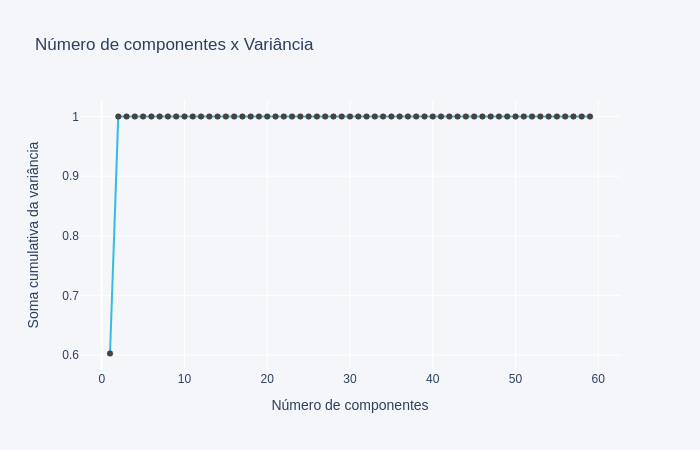
\includegraphics[width=1.0\linewidth,clip=true,trim=0cm 0cm 0cm 0cm, keepaspectratio=true]{points_pca_gabor.png}
	\caption{Selecionar o menor número de componentes retendo 100\% de variância.}
	\label{fig:points_pca_gabor}
\end{figure}

Observa-se melhores resultados comparado com o experimento anterior. Pois se fez possível reduzir as características de 60 para duas retendo 100\% de variância. Embora o desempenho dos classificadores atingirem no máximo 69.3\%, nota-se grande melhoria quando é reduzida a quantidade de características quando compara-se os resultados da Figura~\ref{fig:bar_norm_all_gabor} com a Figura~\ref{fig:bar_result_gabor}

\begin{figure}[!htbp]
	\centering
	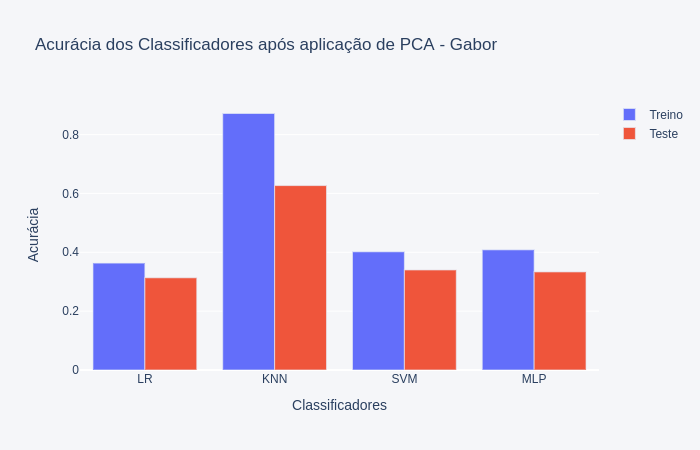
\includegraphics[width=1.0\linewidth,clip=true,trim=0cm 0cm 0cm 0cm, keepaspectratio=true]{bar_result_gabor.png}
	\caption{Acurácia com o descritor Gabor após redução de dimensionalidade}
	\label{fig:bar_result_gabor}
\end{figure}

\section{Resultados}
Nas seções anteriores foram coletados alguns indícios para seleção do descritores combinadas com a melhor técnica de normalização, menor número de características. Por isso, para consolidar os dados anteriores e evitar superestimação dos resultados encontrados foi utilizado a técnica de validação cruzada estratificada em 10 partições.

\subsubsection{Descritor LBP}
Com relação a acurácia as médias e devio padrão foram respectivamente: LR: 69\%, 16\%; KNN: 46\%, 24\%; SVM: 64\%, 22\%; MLP: 71\%, 18\%. Estes dados podem ser vistos na Tabela ~\ref{tab:result_lbp} e Figura~\ref{fig:box_result_lbp}.


\begin{table}[!htbp]
	\caption{Acurácia dos classificadores utilizando o descritor LBP}
	\begin{center}
		\begin{tabular}{|c|c|c|}
			\hline
			& Média & Desvio Padrão \\
			\hline
			MLP       & 71\% & 18\% \\
			LR        & 69\% & 16\% \\
			SVM       & 64\% & 22\% \\
			KNN       & 46\% & 24\% \\
			\hline
		\end{tabular}
		\label{tab:result_lbp}
	\end{center}
\end{table}

\begin{figure}[!htbp]
	\centering
	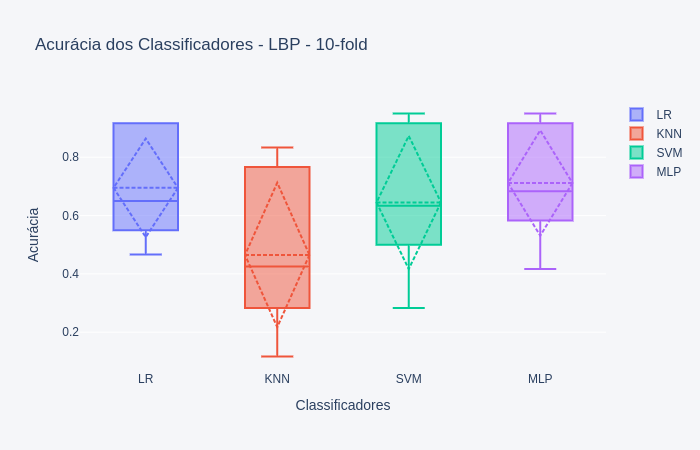
\includegraphics[width=1.0\linewidth,clip=true,trim=0cm 0cm 0cm 0cm, keepaspectratio=true]{box_result_lbp.png}
	\caption{Média e Desvio Padrão da Acurácia com o descritor LBP}
	\label{fig:box_result_lbp}
\end{figure}

\subsubsection{Descritor Gabor}
Com o descritor Gabor a média e desvio padrão foram respectivamente: LR: 28\%, 26\%; KNN: 25\%, 13\%; SVM: 29\%, 30\%; MLP: 27\%, 28\%.. Estes dados podem ser vistos na Tabela ~\ref{tab:result_gabor} e Figura~\ref{fig:box_result_gabor}. 


\begin{table}[!htbp]
	\caption{Acurácia dos classificadores utilizando o descritor Gabor}
	\begin{center}
		\begin{tabular}{|c|c|c|}
			\hline
			& Média & Desvio Padrão \\
			\hline
			SVM       & 29\% & 30\% \\
			LR        & 28\% & 26\% \\
			MLP       & 27\% & 28\% \\
			KNN       & 25\% & 13\% \\
			\hline
		\end{tabular}
		\label{tab:result_gabor}
	\end{center}
\end{table}

\begin{figure}[!htbp]
	\centering
	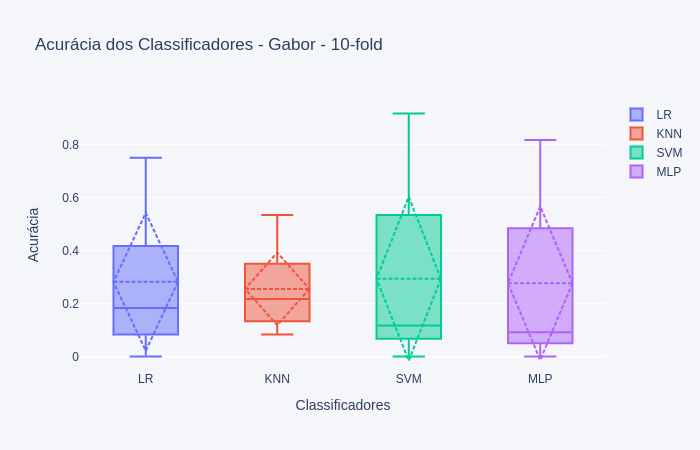
\includegraphics[width=1.0\linewidth,clip=true,trim=0cm 0cm 0cm 0cm, keepaspectratio=true]{box_result_gabor.png}
	\caption{Média e Desvio Padrão da Acurácia com o descritor Gabor}
	\label{fig:box_result_gabor}
\end{figure}

\section{CONCLUSÃO E TRABALHOS FUTUROS}
Neste trabalho foi realizado o reconhecimento de expressões faciais com aprendizado de máquina. Foram comparadas com base na acurácia o melhor desempenho para os descritores LBP e Gabor. O primeiro foi que obteve melhor resultado. Foram comparadas diferentes técnicas de normalização sendo que os testes realizados com o descritor Gabor foi o que apresentou maior sensibilidade para este tipo de alteração. Além disto foi aplicada a técnica de redução de dimensionalidade com o PCA, novamente os resultados baseados no descritor Gabor foi o mais afetado.

Por fim, coletou-se os indícios de qual a combinação de descritor, técnica de escalonamento, redução de dimensionalidade realizamos a validação cruzadada estratificada para obter estimativas mais precisas. Com isto ocorreu notável queda no desempenho dos classificadores.

Como trabalhos futuros pode-se buscar novas bases de imagens. Identificar regiões das faces específicas e extrair as características manualmente com os filtros utilizados para ser possível a regulação dos parâmetros do filtro Gabor e LBP. Com relação aos classificadores utilizar Grid Search e validação cruzada para selecionar os parâmetros exigidos pelos algorítmos de classificação utilizados. Pode-se também utilizar algorítmos de \textit{Deep learning}.



\bibliography{referencias}
\bibliographystyle{plain}

\end{document}
